
\textbf{\huge{Résumé}}\\[4cm]
\begin{center}
Certaines pathologies visuelles, principalement d'origine dégénérative, sont incurables. Elles conduisent souvent à une déficience visuelle, parfois à la cécité. Cette déficience visuelle
handicape la personne dans toute sa vie en diminuant son efficacité dans ses activités quotidiennes, en augmentant les risques de chutes ou d'accidents, en la coupant peu à peu
de toute vie sociale, culturelle et parfois même familiale... En plus du problème de la vision, il y a un véritable problème humain.
Face à ce constat, notre projet a développé des lunettes intelligentes pour les malvoyants dont le principe est d'aider le malvoyant à entendre ce qu'il veut voir. En termes techniques, ces lunettes intelligentes vont convertir le contenu d'une image ou d'une vidéo en un fichier audio. \\[1cm]
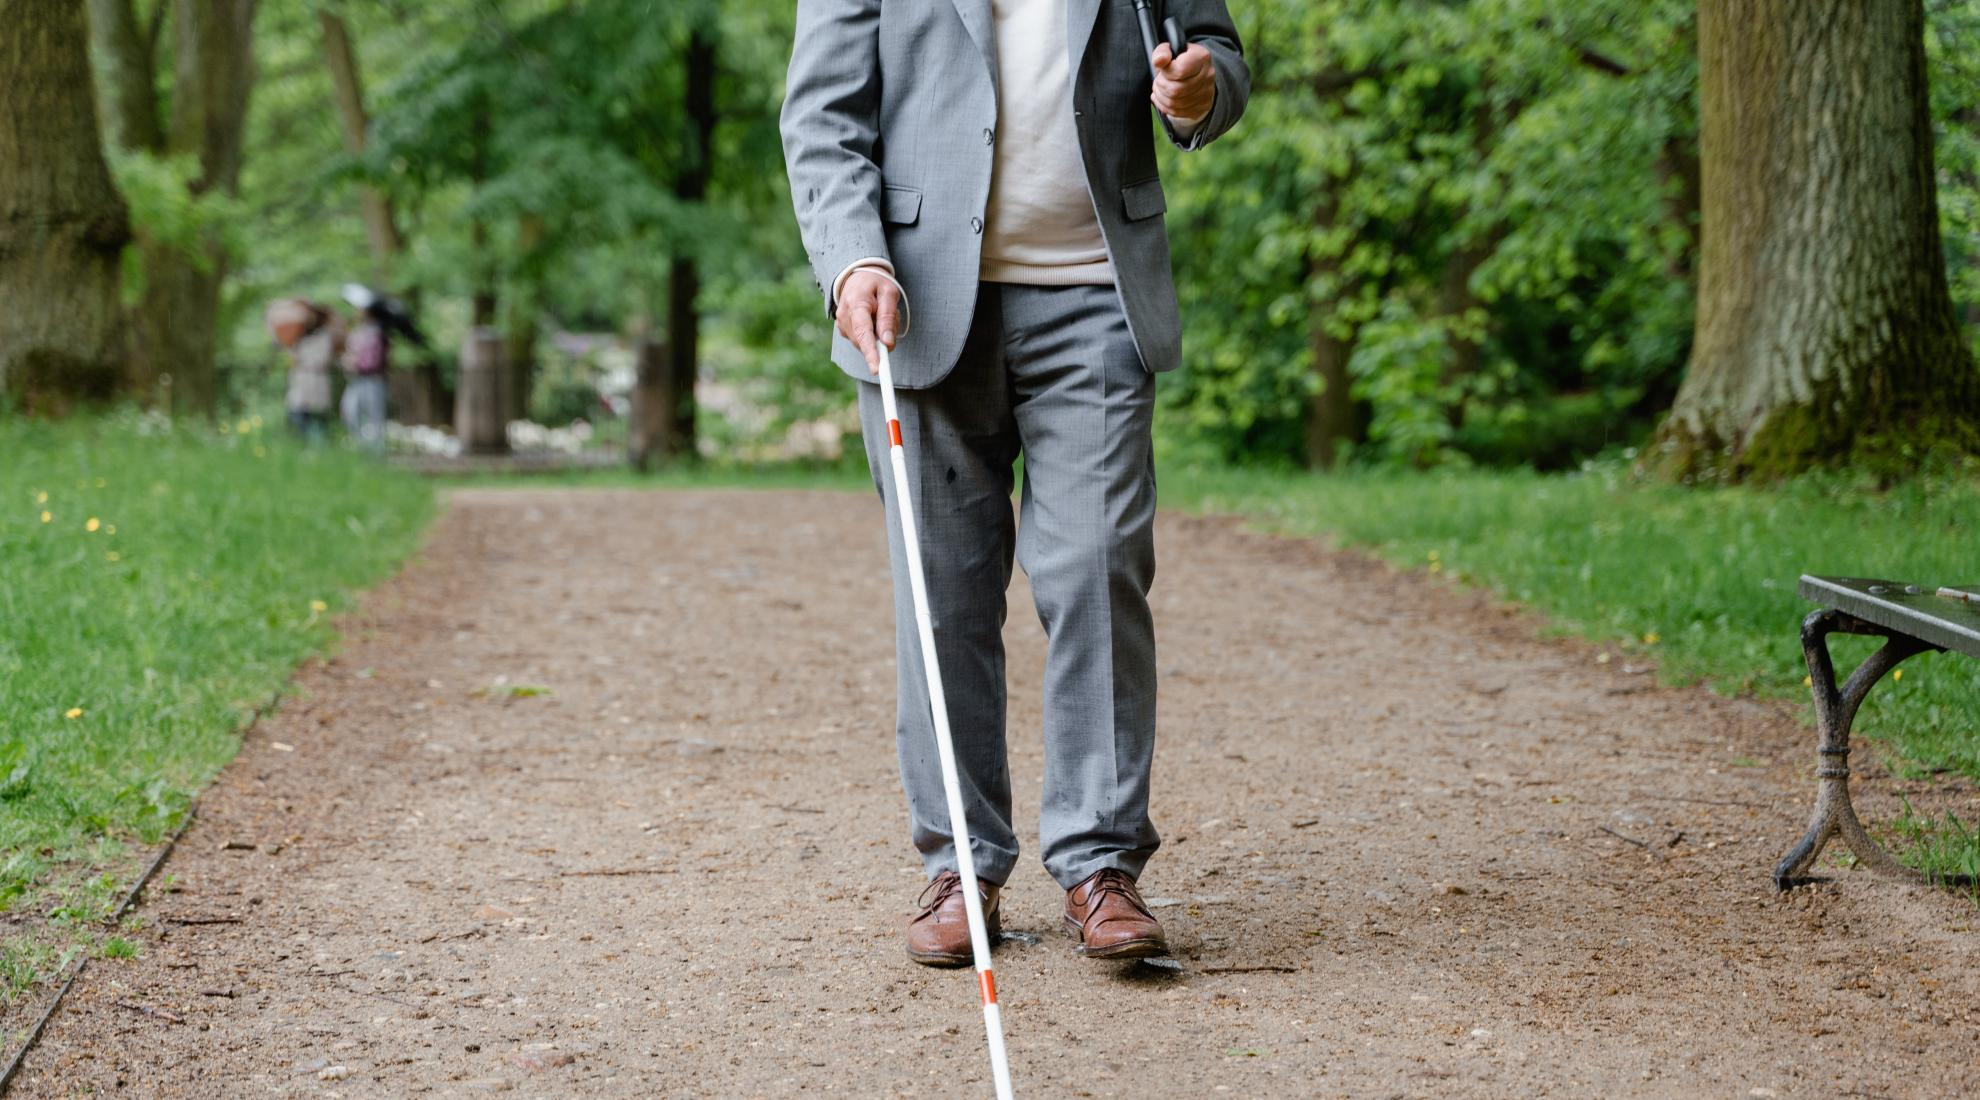
\includegraphics[width=14cm, height=7cm]{4-Images/visually-impaired.jpeg}\\[2cm]
\end{center}
